\documentclass{article}

%package setup
\usepackage{graphicx}
\usepackage{amsmath}
\usepackage{fancyhdr}
\usepackage[margin=1in]{geometry}
\usepackage{comment}
\usepackage{placeins}
\usepackage{parskip}
\usepackage{subcaption}
\usepackage{appendix}
\usepackage{soul}
\usepackage{comment}
\usepackage[hidelinks]{hyperref}
\usepackage{matlab-prettifier}
\usepackage{minted}
\usepackage{enumitem}
\usepackage{float}
\usepackage{textcomp, gensymb}
\usepackage{caption}

\pagestyle{fancy}
\fancyhf{} % Clear header/footer settings
\rhead{\thepage} % Page number on the right in the header
\lhead{ASE375 Lab Report 5} % Your lab report title on the left

\begin{document}

\begin{titlepage}
  \centering
  
\includegraphics[width=10cm]{ase-logo-formal.png}  % Adjust the width as needed
  \vspace{1cm}  % Add some vertical space
 
  \Large \textbf{ASE 375 Electromechanical Systems}\\
  \large \textbf{Section 14115}\\
  \vspace{0.5cm}
  \textbf{Monday: 3:00 - 6:00 pm}\\
 
  \vspace{1cm}
 
  \hrule
  \vspace{0.5cm}
 
  \Huge \textbf{Report 5:\\
  Strain-gage Measurements and Fourier Analysis}\\
  \Huge \textbf{}\\
 
  \vspace{0.5cm}
  \hrule
 
  \vspace{1cm}
 
  \normalsize \textbf{Andrew Doty, Andres Suniaga, Dennis Hom}\\
  \normalsize \textbf{Due Date: 03/18/2024}
 
\end{titlepage}
\newpage

\tableofcontents
\thispagestyle{empty}
\newpage

\section{Introduction}
This experiment presents results of strain-gage measurements performed at the root of a cantilever beam undergoing (1) Different weights placed at its tip and (2) An applied force which leaves the beam freely vibrating. The purpose of this experiment is to learn about the Wheatstone bridge configurations in gathering our strain-gage data on the beam and how different sampling frequencies affect these strain measurements.
\vspace{5mm}

In (1), results of strain measurements at the root of the beam are gathered using two different half-bridge configurations. Using the Euler-Bernoulli Beam theory, we make comparisons between the ideal and real strain-gage results. In (2), we model the strain as a function of time at different sampling frequencies. For (2), we utilize one of the half-bridge configurations and perform Fourier analysis to estimate the natural frequency of the cantilever beam. 

\section{Equipment}
Measurement devices and hardware used in this lab include:
\begin{itemize}

\item Cantilever Beam: 
\vspace{1mm}

A uniform aluminum beam that is cantilevered at one end (root) with a string attached at the other end (tip) for holding weights.
\vspace{2.5mm}

\begin{figure}[H]
    \centering
    \caption*{Side View}
    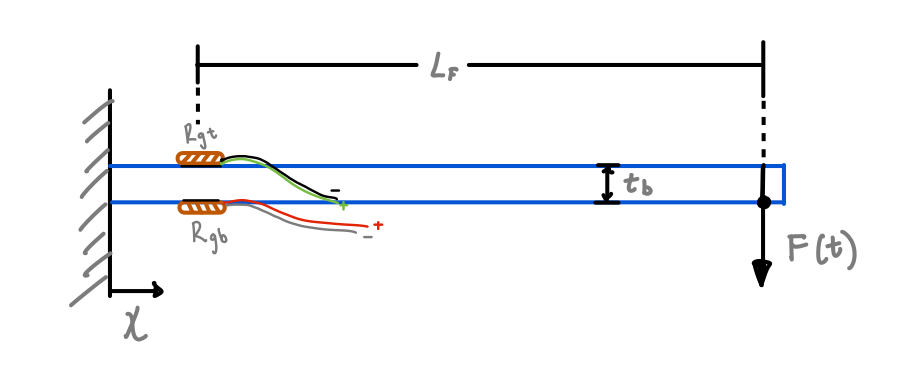
\includegraphics[width = 0.7\textwidth]{cantilever_sideview.png}
\end{figure}
\begin{figure}[H]
    \centering
    \caption*{Top View}
    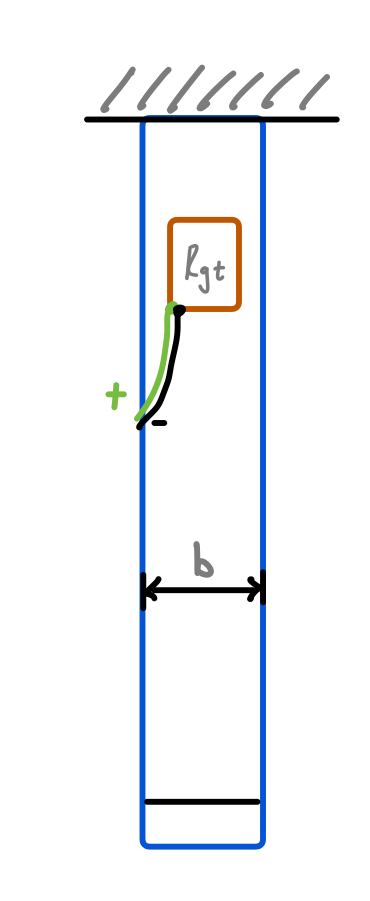
\includegraphics[width = 0.15\textwidth]{cantilever_topview.png}
\end{figure}

\item Digital Calipers, $\epsilon_{b} = 0.005\; \text{mm}$: 
\vspace{1mm}

Used for measuring outer and inner dimensions of objects. In our case we use it to the measure the wall thickness, $t_{b}$, and width, $b$, of the cantilever beam.
\vspace{2.5mm}

\item Ruler/Tape Measure, $\epsilon_{b} = 0.5\; \text{mm}$: 
\vspace{1mm}

Used to measure the length of the cantilever beam, $L_{F}$.
\vspace{2.5mm}

\item Brass Slotted Weights with hanger: 
\vspace{1mm}

Used to induce bending on the tip of the cantilever beam to acquire strain measurements. Hanger is $50\; \text{g}$ along with ten $20\; \text{g}$ weights. Total $250$ grams. 
\vspace{2.5mm}

\item Strain Gauge: 
\vspace{1mm}

Sensor used to measure surface strains which then converts it into a change in electrical resistance. An output voltage is produced when a surface strain occurs since there is a resistance change within the bridge configuration.
\vspace{1mm}

In this lab, we have 2 strain gauges placed at the root of the cantilever beam. One of them is on the top surface of the beam, $R_{g t}$, and the other is placed on the bottom surface, $R_{g b}$.
\vspace{2.5mm}

\item DAQ, NI-9215 Voltage Input Module, and LabVIEW:
\vspace{1mm}

Data Acquisition System used to process sample measurements into digital data. NI-9215 is an analog input module used to measure the output voltage signals of sensors and send it through the DAQ system. LabVIEW used to model these output voltages read from the DAQ of the strain-gage measurements. We connect to the $5 \text{V}$ port of the DAQ for our experiment.
\vspace{2.5mm}

\item Solderless Breadboard, Jumper Wires, and $350\Omega$ Resistors: 
\vspace{1mm}

Used to make connections to the input analog modules and to construct circuits. In this lab we build two configurations of the Wheatstone half-bridge circuit with two $350\Omega$ dummy resistors, labeled $R_{D}$, and the two strain gauges, $R_{gt}$ and $R_{gb}$. Configurations are shown below, with an example of the configuration B circuit on the breadboard:

\hypertarget{fig1}{}
\begin{figure}[H]
    \centering
    \frame{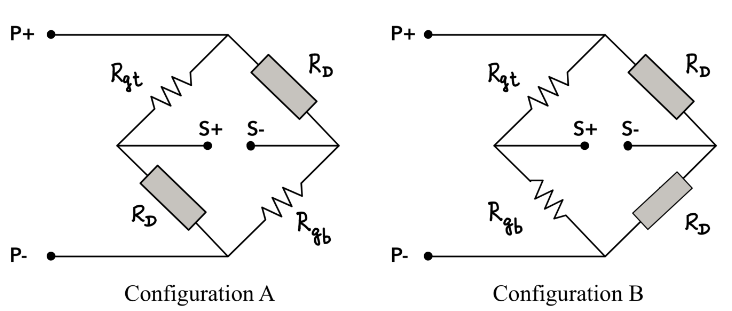
\includegraphics[width = 0.5\textwidth]{Half_bridge_configs.png}}
    \caption{Half-Bridge Configurations, $V_{OUT}$ between $S^{+}$ and $S^{-}$}
\end{figure}
\begin{figure}[H]
    \centering
    \frame{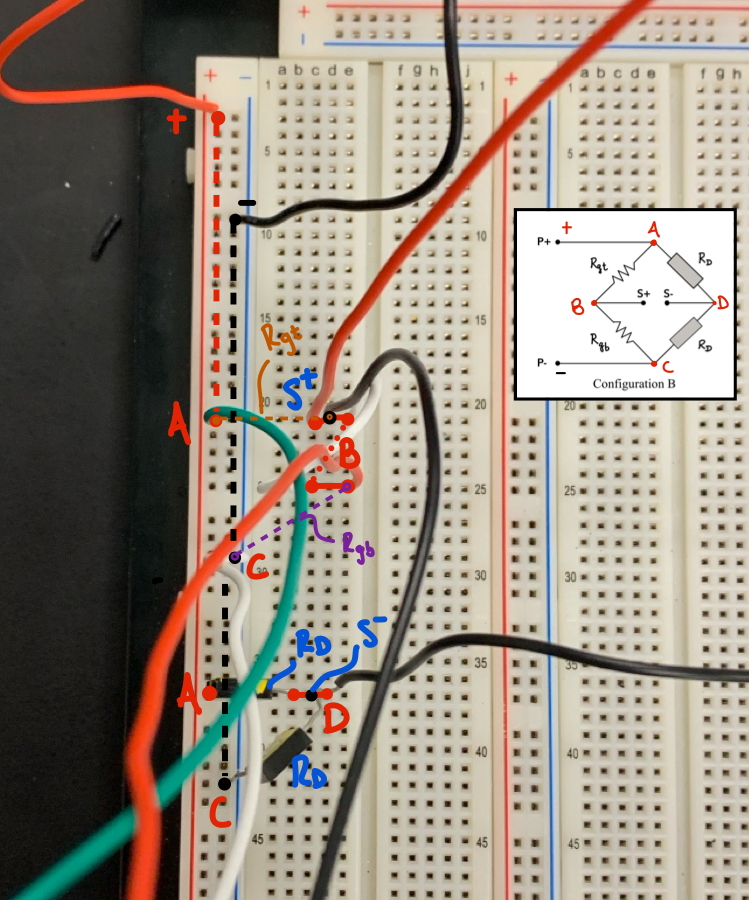
\includegraphics[width = 0.75\textwidth]{configB_circuit.png}}
    \caption{Configuration B Half-Bridge Circuit on the Breadboard}
\end{figure}

To switch from Configuration B to Configuration A, rearrange connections at $B$ and $D$ such that the dummy resistor from $\overrightarrow{DC}$ is now $\overrightarrow{BC}$ and bring the positive wire of the bottom strain-gage, $R_{gb}$, from $B$ to $D$.


\end{itemize}

\section{Procedure}
This experiment is broken up into two parts. In Part 1, we will be gathering the average output voltage read from the two half-bridge configurations as shown in \hyperlink{fig1}{Figure 1} as weights hanging off the tip of the cantilever beam. In Part 2, we will be testing different sampling frequencies and collecting the output voltage read from the half-bridge circuit following Configuration B as the beam undergoes free vibration as a result of an applied force at the tip. 
\vspace{2.5mm}

Before experimenting, we must set up the LabVIEW model following the form:
\begin{figure}[H]
    \centering
    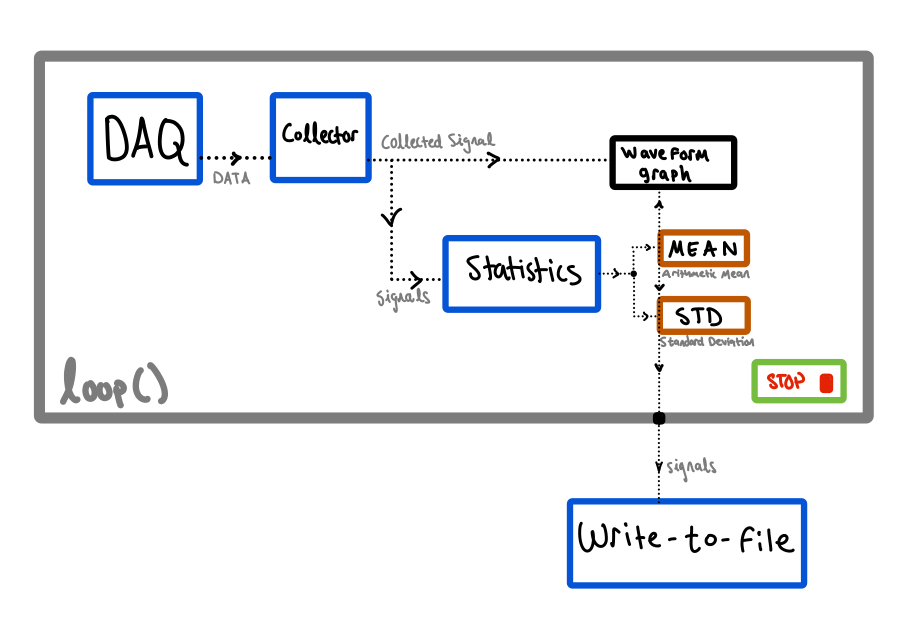
\includegraphics[width = 0.85\textwidth]{labview_blockdiagram.png}
    \caption{LabVIEW Block Diagram for modeling $V_{OUT}=f(t)$}
\end{figure}

The Write-to-File block will be used for Part 2 as we model the strain and output voltage as a function of time.

\subsection{Part 1}
\begin{enumerate}
    \item Create the half-bridge circuit following Configuration A as shown in \hyperlink{fig1}{Figure 1}. 
    \item Verify that the output is modeled correctly through LabVIEW by applying force to the beam. Once the setup is working well continue to the next step.
    \item Begin with no weight hanging at the tip of the beam. This is the "zero" reading. Once the output stabilizes, note down the mean and standard deviation of $V_{OUT}$.
    \item Continue collecting the output readings at each weight (in grams) as follows:
    \vspace{0.5mm}
    
    $\textbf{W}_{\text{up}} = \left[0,\, 50,\, 90,\, 130,\, 170,\, 210,\, 250\right]$. 
    \begin{itemize}
        \item $\textbf{W}_{\text{up}}$ is the sequence we follow as we add weight to the tip of the beam. We have already collected the $0\, \text{g}$ reading so the next one is adding the hanger which weighs $50\, \text{g}$. We then go up by two $20\, \text{g}$ weights until we reach the total $250\, \text{g}$.
    \end{itemize}
    
    \item Now repeat step 3 as go down in weight, which follows the sequence:
    \vspace{0.5mm}
    
    $\textbf{W}_{\text{down}} = \left[230,\, 210,\, 190,\, 170,\, 150,\, 130,\, 110,\, 90,\, 70,\, 50,\, 0\right]$.
    \begin{itemize}
        \item We record the output reading as we remove one $20\, \text{g}$ at a time until there is no more weight. 
    \end{itemize}

    \item Switch to the half-bridge circuit following \underline{Configuration B} as shown in \hyperlink{fig1}{Figure 1} and \ul{repeat steps 2 through 5}.

    \item We note down our observations and begin \hyperlink{datapro}{\textbf{Data Processing}} to model the strain as we loaded and unloaded the beam with weights.
\end{enumerate}

\subsection{Part 2}
In this part, we will be utilizing the write-to-file block to collect our data through time. Instead of adding weight to the tip of the beam, we will flick the tip of the beam so it will freely oscillate up and down.

\begin{enumerate}
    \item Use the half-bridge circuit following Configuration B as shown in \hyperlink{fig1}{Figure 1}. 
    \item In LabVIEW, we can change the sampling frequency, $f_{S}$, and number of samples collected, $N$, by going into the DAQ and Collector block. We will collect output voltage readings through this sequence of sampling frequencies:
    \vspace{0.5mm}

    \(\textbf{f}_{S} = \left[10,\, 20,\, 50,\, 100,\, 1000\right]\; \text{Hz}\)

    \item For each $f_{S_{i}}$, run the sampling model on LabVIEW and apply a force at the tip of the beam so that it will freely oscillate until the sampling reaches its end. Stop and Save the sample data.

    \item Once finished, note down observations of the effects of different sampling frequencies and continue to \hyperlink{datapro}{\textbf{Data Processing}} to do time-frequency analysis and find the natural frequency, $f_{N}$, of the cantilevered aluminum beam.
\end{enumerate}

\hypertarget{datapro}{}
\section{Data Processing}
\subsection{Variables and Equations}
\begin{enumerate}[label = \Roman*.]
    \item 
\end{enumerate}
\section{Results and Analysis}

\section{Conclusion}

\newpage
\thispagestyle{empty}  % Clear header/footer
\begin{center}
	\vspace*{\fill}
	{\Huge Appendices}
	\vspace*{\fill}
\end{center}

% Start appendices
\newpage
\begin{appendices}
\pagestyle{fancy}
\renewcommand{\thefigure}{A\arabic{figure}}
\setcounter{figure}{0}

% \section*{t-Distribution Tables}
% \hypertarget{1}{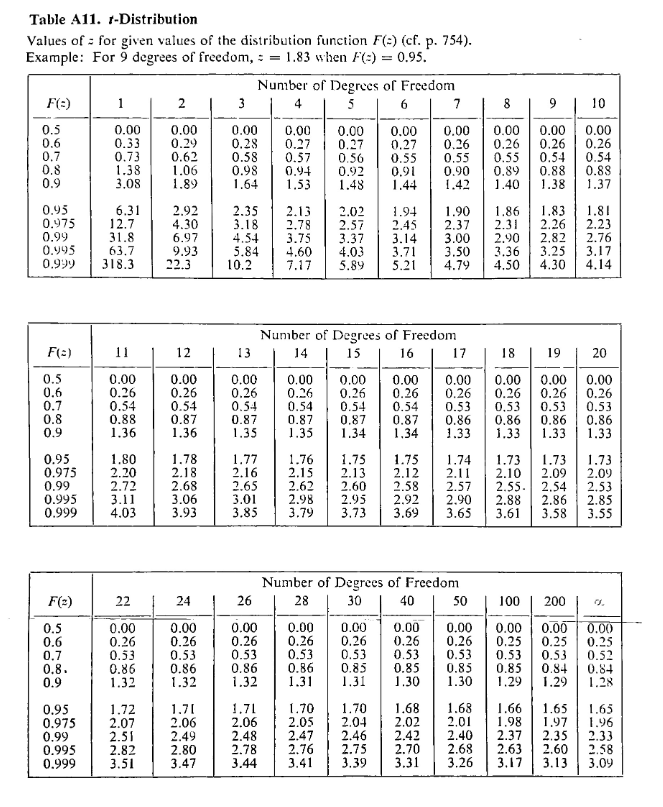
\includegraphics[width=0.95\textwidth]{t_distribution_Table_lecture3.png}}

\section*{NI-9215 Datasheet}
\url{https://www.amc-systeme.de/files/pdf/ni-9215-amc.pdf}

\end{appendices}

\end{document}
